\documentclass[]{article}
\usepackage[T1]{fontenc}
\usepackage{lmodern}
\usepackage{amssymb,amsmath}
\usepackage{ifxetex,ifluatex}
\usepackage{fixltx2e} % provides \textsubscript
% use microtype if available
\IfFileExists{microtype.sty}{\usepackage{microtype}}{}
\ifnum 0\ifxetex 1\fi\ifluatex 1\fi=0 % if pdftex
  \usepackage[utf8]{inputenc}
\else % if luatex or xelatex
  \usepackage{fontspec}
  \ifxetex
    \usepackage{xltxtra,xunicode}
  \fi
  \defaultfontfeatures{Mapping=tex-text,Scale=MatchLowercase}
  \newcommand{\euro}{€}
\fi
% Redefine labelwidth for lists; otherwise, the enumerate package will cause
% markers to extend beyond the left margin.
\makeatletter\AtBeginDocument{%
  \renewcommand{\@listi}
    {\setlength{\labelwidth}{4em}}
}\makeatother
\usepackage{enumerate}
\usepackage{ctable}
\usepackage{float} % provides the H option for float placement
\usepackage{graphicx}
% We will generate all images so they have a width \maxwidth. This means
% that they will get their normal width if they fit onto the page, but
% are scaled down if they would overflow the margins.
\makeatletter
\def\maxwidth{\ifdim\Gin@nat@width>\linewidth\linewidth
\else\Gin@nat@width\fi}
\makeatother
\let\Oldincludegraphics\includegraphics
\renewcommand{\includegraphics}[1]{\Oldincludegraphics[width=\maxwidth]{#1}}
\ifxetex
  \usepackage[setpagesize=false, % page size defined by xetex
              unicode=false, % unicode breaks when used with xetex
              xetex]{hyperref}
\else
  \usepackage[unicode=true]{hyperref}
\fi
\hypersetup{breaklinks=true,
            bookmarks=true,
            pdfauthor={},
            pdftitle={},
            colorlinks=true,
            urlcolor=blue,
            linkcolor=magenta,
            pdfborder={0 0 0}}
\setlength{\parindent}{0pt}
\setlength{\parskip}{6pt plus 2pt minus 1pt}
\setlength{\emergencystretch}{3em}  % prevent overfull lines

\author{}
\date{}

\begin{document}

{
\hypersetup{linkcolor=black}
\tableofcontents
}
\section{State-of-the-Art in Group Elicitation Strategies}

This section presents the main elicitation or aggregation strategies
being used in GRecSys. {[}@masthoff11group{]} The purpose of them are to
adapt to the group as a whole based on information about individual
users' likes and dislikes (i.e.: aggregating individual ratings into a
group rating).

\begin{figure}[htbp]
\centering
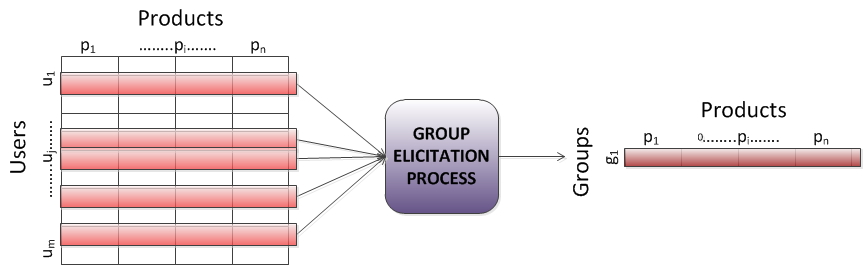
\includegraphics{./img/ElicitationTechs.png}
\caption{Elicitation Process}
\end{figure}

Veure imatge de {[}Gartrell, M., Xing, X., Lv, Q., Beach, A., Han, R.,
Mishra, S., \& Seada, K. (2010). Enhancing group recommendation by
incorporating social relationship interactions. Proceedings of the 16th
ACM international conference on Supporting group work (pp.~97--106). New
York, NY, USA: ACM. doi:10.1145/1880071.1880087{]}

\begin{center}\rule{3in}{0.4pt}\end{center}

{[}@Senot:2011:EGP:2283696.2283850{]}

There exist two main approaches for providing recommendations to a group
of users when the ``real'' group profile is not available. 1. The first
combines individual recommendations to generate a list of group
recommendations, 2. while the second computes group recommendations
using a group profile derived from individual profiles.

\begin{itemize}
\item
  The majority-based strategies use the ``most popular'' choices (user
  preferences, item rankings, etc.) among group members.
\end{itemize}

For example, GroupCast {[}McCarthy et al., 2001{]} displays content that
suits the intersection of user profiles when the people are close to a
public screen.

\emph{Plurality Voting}, \emph{Borda Count}, \emph{Copeland Rule} ,
\emph{Approval Voting}

\begin{itemize}
\item
  The consensus-based strategies consider the preferences of all group
  members.
\end{itemize}

Examples include the \emph{Utilitarian strategy} which averages the
preferences of all the group members, the \emph{Fairness strategy}, or
the \emph{Alternated Satisfaction strategy}.

As an example, MusicFX {[}McCarthy and Anagnost, 1998{]} recommends the
most relevant music station in a fitness center using a group profile
computed by summing the squared individual preferences. By applying this
strategy 71\% of clients noticed a positive difference (as compared to
the absence of the recommendation system).

\emph{Median}, \emph{Average}, \emph{Additive}, \emph{Average without
Misery}, \emph{Fairness} and \emph{Multiplicative}

\begin{itemize}
\item
  The borderline strategies, also called role-based strategies, consider
  only a subset of items (item categories) in individual profiles, based
  on user roles or any other relevant criteria.
\end{itemize}

\emph{Least Misery}, \emph{Most Pleasure}, \emph{Most respected person}

For example, PolyLens {[}O'Connor et al., 2001{]} uses the Least Misery
strategy to recommend movies for small user groups based on the
MovieLens database (http://www.movielens.org). Their survey showed that
77\% of PolyLens users found group recommendations more helpful than
individual ones. Yet this system only works with a single strategy.

\begin{center}\rule{3in}{0.4pt}\end{center}

\subsection{Overview}

Eleven aggregation strategies inspired by Social Choice Theory are
summarized in Table 3 (see {[}17{]} for more details).

\ctable[caption = {Example of individual ratings for ten items (A to
J)}, pos = H, center, botcap]{lcccccccccc}
{% notes
}
{% rows
\FL
\parbox[b]{0.10\columnwidth}{\raggedright
} & \parbox[b]{0.06\columnwidth}{\centering
A
} & \parbox[b]{0.06\columnwidth}{\centering
B
} & \parbox[b]{0.06\columnwidth}{\centering
C
} & \parbox[b]{0.06\columnwidth}{\centering
D
} & \parbox[b]{0.06\columnwidth}{\centering
E
} & \parbox[b]{0.06\columnwidth}{\centering
F
} & \parbox[b]{0.06\columnwidth}{\centering
G
} & \parbox[b]{0.06\columnwidth}{\centering
H
} & \parbox[b]{0.06\columnwidth}{\centering
I
} & \parbox[b]{0.06\columnwidth}{\centering
J
}
\ML
\parbox[t]{0.10\columnwidth}{\raggedright
Peter Jane Mary
} & \parbox[t]{0.06\columnwidth}{\centering
10 1 10
} & \parbox[t]{0.06\columnwidth}{\centering
4 9 5
} & \parbox[t]{0.06\columnwidth}{\centering
3 8 2
} & \parbox[t]{0.06\columnwidth}{\centering
6 9 7
} & \parbox[t]{0.06\columnwidth}{\centering
10 7 9
} & \parbox[t]{0.06\columnwidth}{\centering
9 9 8
} & \parbox[t]{0.06\columnwidth}{\centering
6 6 5
} & \parbox[t]{0.06\columnwidth}{\centering
8 9 6
} & \parbox[t]{0.06\columnwidth}{\centering
10 3 7
} & \parbox[t]{0.06\columnwidth}{\centering
8 8 6
}
\LL
}

\ctable[caption = {Overview of Aggregation Strategies},
pos = H, center, botcap]{lll}
{% notes
}
{% rows
\FL
\parbox[b]{0.17\columnwidth}{\raggedright
Strategy
} & \parbox[b]{0.41\columnwidth}{\raggedright
How it works
} & \parbox[b]{0.41\columnwidth}{\raggedright
Example
}
\ML
\parbox[t]{0.17\columnwidth}{\raggedright
\emph{Plurality Voting}
} & \parbox[t]{0.41\columnwidth}{\raggedright
Uses `first past the post': repetitively, the item with the most votes
is chosen.
} & \parbox[t]{0.41\columnwidth}{\raggedright
A is chosen first, as it has the highest rating for the majority of the
group, followed by E (which has the highest rating for the majority when
excluding A).
}
\\\noalign{\medskip}
\parbox[t]{0.17\columnwidth}{\raggedright
\emph{Median}
} & \parbox[t]{0.41\columnwidth}{\raggedright
Middle value of individual ratings
} & \parbox[t]{0.41\columnwidth}{\raggedright
B's group rating is \texttt{5}, from \texttt{(4,9,5)}.
}
\\\noalign{\medskip}
\parbox[t]{0.17\columnwidth}{\raggedright
\emph{Average} or \emph{Utilitarian}
} & \parbox[t]{0.41\columnwidth}{\raggedright
Averages individual ratings
} & \parbox[t]{0.41\columnwidth}{\raggedright
B's group rating is \texttt{6}, namely \texttt{(4+9+5)/3}.
}
\\\noalign{\medskip}
\parbox[t]{0.17\columnwidth}{\raggedright
\emph{Additive}
} & \parbox[t]{0.41\columnwidth}{\raggedright
Adds individual ratings
} & \parbox[t]{0.41\columnwidth}{\raggedright
B's group rating is \texttt{18}, namely \texttt{4+9+5}.
}
\\\noalign{\medskip}
\parbox[t]{0.17\columnwidth}{\raggedright
\emph{Multiplicative}
} & \parbox[t]{0.41\columnwidth}{\raggedright
Multiplies individual ratings
} & \parbox[t]{0.41\columnwidth}{\raggedright
B's group rating is \texttt{180}, namely \texttt{4*9*5}.
}
\\\noalign{\medskip}
\parbox[t]{0.17\columnwidth}{\raggedright
\emph{Borda Count}
} & \parbox[t]{0.41\columnwidth}{\raggedright
Counts points from items' rankings in the individuals' preference lists,
with bottom item getting 0 points, next one up getting one point, etc
} & \parbox[t]{0.41\columnwidth}{\raggedright
A's group rating is \texttt{17}, namely \texttt{0} (last for Jane)
\texttt{+ 9} (first for Mary) \texttt{+ 8} (shared top 3 for Peter)
}
\\\noalign{\medskip}
\parbox[t]{0.17\columnwidth}{\raggedright
\emph{Copeland Rule}
} & \parbox[t]{0.41\columnwidth}{\raggedright
Counts how often an item beats other items (using majority vote) minus
how often it looses
} & \parbox[t]{0.41\columnwidth}{\raggedright
F's group rating is \texttt{5}, as F beats 7 items (B,C,D,G,H,I,J) and
looses from 2 (A,E).
}
\\\noalign{\medskip}
\parbox[t]{0.17\columnwidth}{\raggedright
\emph{Approval Voting}
} & \parbox[t]{0.41\columnwidth}{\raggedright
Counts the individuals with ratings for the item above a approval
threshold (e.g.~6)
} & \parbox[t]{0.41\columnwidth}{\raggedright
B's group rating is \texttt{1} and F's is \texttt{3}.
}
\\\noalign{\medskip}
\parbox[t]{0.17\columnwidth}{\raggedright
\emph{Least Misery}
} & \parbox[t]{0.41\columnwidth}{\raggedright
Takes the minimum of individual ratings
} & \parbox[t]{0.41\columnwidth}{\raggedright
B's group rating is \texttt{4}, namely the smallest of \texttt{4,9,5}.
}
\\\noalign{\medskip}
\parbox[t]{0.17\columnwidth}{\raggedright
\emph{Most Pleasure}
} & \parbox[t]{0.41\columnwidth}{\raggedright
Takes the maximum of individual ratings
} & \parbox[t]{0.41\columnwidth}{\raggedright
B's group rating is \texttt{9}, namely the largest of \texttt{4,9,5}.
}
\\\noalign{\medskip}
\parbox[t]{0.17\columnwidth}{\raggedright
\emph{Average without Misery}
} & \parbox[t]{0.41\columnwidth}{\raggedright
Averages individual ratings, after excluding items with individual
ratings below a certain threshold (say 4).
} & \parbox[t]{0.41\columnwidth}{\raggedright
J's group rating is \texttt{7.3} (the average of \texttt{8,8,6}), while
A is excluded because Jane hates it.
}
\\\noalign{\medskip}
\parbox[t]{0.17\columnwidth}{\raggedright
\emph{Fairness}
} & \parbox[t]{0.41\columnwidth}{\raggedright
Items are ranked as if individuals are choosing them in turn.
} & \parbox[t]{0.41\columnwidth}{\raggedright
Item E may be chosen first (highest for Peter), followed by F (highest
for Jane) and A (highest for Mary).
}
\\\noalign{\medskip}
\parbox[t]{0.17\columnwidth}{\raggedright
\emph{Most respected person}
} & \parbox[t]{0.41\columnwidth}{\raggedright
Uses the rating of the most respected individual.
} & \parbox[t]{0.41\columnwidth}{\raggedright
If Jane is the most respected person, then A's group rating is
\texttt{1}. If Mary is most respected, then it is \texttt{10}.
}
\LL
}

\ctable[caption = {Overview of Aggregation Strategies},
pos = H, center, botcap]{ll}
{% notes
}
{% rows
\FL
Strategy & Example Ranked List
\ML
\emph{Plurality
Voting} & $\lbrace i_{5}, i_{6}, i_{4}, i_{8}, i_{10}, i_{1}, i_{9}, i_{2}, i_{7}, i_{3}\rbrace$
\\\noalign{\medskip}
\emph{Median} & $\lbrace i_{1},i_{5}-i_{6},i_{8}-i_{10},i_{4}-i_{9},i_{7},i_{2},i_{3}\rbrace$
\\\noalign{\medskip}
\emph{Average} & $\lbrace i_{5}-i_{6}, i_{8}, i_{4}-i_{10}, i_{1}, i_{9}, i_{2}, i_{7}, i_{3}\rbrace$
\\\noalign{\medskip}
\emph{Additive} & $\lbrace i_{5}-i_{6}, i_{8}, i_{4}-i_{10}, i_{1}, i_{9}, i_{2}, i_{7}, i_{3}\rbrace$
\\\noalign{\medskip}
\emph{Multiplicative} & $\lbrace i_{6}, i_{5}, i_{8}, i_{10}, i_{4}, i_{9}, i_{2}-i_{7}, i_{1}, i_{3}\rbrace$
\\\noalign{\medskip}
\emph{Borda
Count} & $\lbrace i_{6}, i_{5}, i_{1}, i_{4}-i_{8}, i_{9}, i_{10}, i_{2}, i_{7}, i_{3}\rbrace$
\\\noalign{\medskip}
\emph{Copeland
Rule} & $\lbrace i_{5}, i_{1}, i_{6}, i_{9}, i_{4}, i_{8}, i_{10}, i_{2}-i_{7}, i_{3}\rbrace$
\\\noalign{\medskip}
\emph{Approval
Voting} & $\lbrace i_{4}-i_{5}-i_{6}-i_{8}-i_{10}, i_{1}-i_{7}-i_{9}, i_{2}-i_{3}\rbrace$
\\\noalign{\medskip}
\emph{Least
Misery} & $\lbrace i_{6}, i_{5}, i_{4}-i_{8}-i_{10}, i_{7}, i_{2}, i_{9}, i_{3}, i_{1}\rbrace$
\\\noalign{\medskip}
\emph{Most
Pleasure} & $\lbrace i_{1}-i_{5}-i_{9}, i_{2}-i_{4}-i_{6}-i_{8}, i_{3}-i_{10}, i_{7}\rbrace$
\\\noalign{\medskip}
\emph{Average Without
Misery} & $\lbrace i_{5}-i_{6}, i_{8}, i_{4}-i_{10},i_{2}, i_{7}\rbrace$
\\\noalign{\medskip}
\emph{Fairness} & $\lbrace i_{5}, i_{6}, i_{4}, i_{8}, i_{10}, i_{7}, i_{1}, i_{2}, i_{9}, i_{3}\rbrace$
\\\noalign{\medskip}
\emph{Purity} & $\lbrace i_{6}, i_{5}, i_{8}, i_{10}, i_{4}, i_{9}, i_{7}, i_{1}, i_{2}, i_{3}\rbrace$
\\\noalign{\medskip}
\emph{Completeness} & $\lbrace i_{6}, i_{5}, i_{8}, i_{10}, i_{4}, i_{9}, i_{1}, i_{2}, i_{7}, i_{3}\rbrace$
\\\noalign{\medskip}
\emph{Logical
Sufficiency} & $\lbrace i_{6}, i_{5}, i_{1}, i_{8}, i_{4}, i_{9}, i_{2}, i_{10}, i_{3}, i_{7}\rbrace$
\\\noalign{\medskip}
\emph{Group
Sufficiency} & $\lbrace i_{6}, i_{7}, i_{10}, i_{8}, i_{4}, i_{5}, i_{2}, i_{3}, i_{9}, i_{1}\rbrace$
\LL
}

\subsection{Detailed description}

The following sections will review theses strategies in detail.

In order to ease the different strategies, a base example is provided:

\begin{center}\rule{3in}{0.4pt}\end{center}

{[}@Salamo:2012:GRC:2339097.2339115{]}

Most well-known strategies used in collaborative filtering algorithms
for recommendation generation.

\begin{enumerate}[1.]
\item
  The Least misery strategy, as defined in Eq. 13, chooses a product
  $p_i$ based on the minimum satisfaction of the individual preferences
\end{enumerate}

The rationale is that a group is as satisfied as its least satisfied
member. --veure formula

\[least_misery(p_i,MI) = arg \min{}\]
\[MSE = \frac{1}{n}\sum_{i}^{n} (p_i - a_i)^2 \]

\begin{enumerate}[1.]
\setcounter{enumi}{1}
\item
  Most pleasure strategy selects the maximum satisfaction of the
  individual preferences, see Eq. 14. It considers that at least one
  member will be maximally satisfied. --veure formula
\end{enumerate}

Previous strategies assume the consensus based on the satisfaction of
one individual: the least or the most satisfied. There is no warranty
that the recommendations will suit the whole group.

\begin{enumerate}[1.]
\setcounter{enumi}{2}
\item
  Multiplicative strategy multiplies the satisfaction of the individual
  users, see Eq. 15. With this strategy, it might happen that a member
  with unique tastes always lose out because their opinion happens to be
  a minority preference.
\end{enumerate}

\begin{center}\rule{3in}{0.4pt}\end{center}

{[}@sweb2012{]}

Though recommendation approaches have addressed group preference
modeling explicitly to a rather limited extent, or in an indirect way in
prior work in the computing field, the related issue of social choice
(also called group decision making, i.e.~deciding what is best for a
group given the opinions of individuals) has been studied extensively in
Economics, Politics, Sociology, and Mathematics {[}24, 33{]}.

The models for the construction of a social welfare function in these
works are similar to the group modeling problem we put forward here.

Other areas in which Social Choice Theory has been studied are
Collaborative Filtering (CF), Meta-search, and Multi-agent systems.

In CF, preferences of a group of individuals are aggregated to produce a
predicted preference for somebody outside the group. Meta-search can be
seen --and formulated-- as a form of group decision making, where the
aggregated inputs are produced by information retrieval systems instead
of people. In a meta-search engine, the rankings produced by multiple
search engines need to be combined into one single list, forming the
well-known problem of rank aggregation in Information Retrieval {[}3{]}.
Ensemble recommenders combining several recommendation algorithms also
involve a particular case of this problem, similarly to meta-search
except for the absence of a query. Finally, in Multi-agent systems,
agents need to take decisions that are not only rational from an
individual's point of view, but also from a social point of view.

In all the above fields, different strategies to combine several users'
preferences and to aggregate item ranking lists can be applied based on
the utilized social welfare function.

These strategies are classified by Senot and colleagues {[}27{]} into
three categories, namely:

\begin{itemize}
\item
  majority-based strategies, which strength the ``most popular'' choices
  (user preferences, item rankings, etc.) among the group, e.g.~Borda
  Count, Copeland Rule, and Plurality Voting strategies;
\item
  consensus-based (or democratic) strategies, which average somehow all
  the available choices, e.g.~Additive Utilitarian, Average without
  Misery, and Fairness strategies;
\item
  and border-line strategies, also called role-based strategies in
  {[}5{]}, which only consider a subset of choices based on user roles
  or any other relevant criterion, e.g.~Dictatorship, Least Misery and
  Most Pleasure strategies.
\end{itemize}

\begin{center}\rule{3in}{0.4pt}\end{center}

In the following, we assume a user has a preference (utility) for each
item represented in the form of a numeric 1-10 rating. In all the cases,
the greater the rating value, the most useful the item is for the user.

\subsubsection{Plurality voting strategy}

Each member votes for his preferred item and the one with the highest
votes is selected. In this strategy, the items that were rated highest
are combined as follows:

\begin{enumerate}[1.]
\item
  A user is randomly selected
\item
  His \emph{L} top rated items are taking into account.

  \begin{itemize}
  \item
    From them, the item that causes the most utility to the group is
    chosen for the group profile with a score equal to \emph{N}, i.e.,
    the number of items.
  \end{itemize}
\item
  Restart the process in step 1 considering the remaining
  \emph{N--1,N--2,etc.} items and uniformly diminishing to 1 the further
  assigned scores.
\end{enumerate}

In the final list, the higher score the more influential the item is for
the group.

\ctable[caption = {Group choice selection following the \emph{plurality
voting strategy}. The ranked list of items for the group would be
$\lbrace i_{5}, i_{6}, i_{4}, i_{8}, i_{10}, i_{1}, i_{9}, i_{2}, i_{7}, i_{3}\rbrace$
following the user selecting order $\lbrace u_{1},u_{2},u_{3}\rbrace$
and $L=3$.}, pos = H, center, botcap]{lllllllllll}
{% notes
}
{% rows
\FL
 & $i_{1}$ & $i_{2}$ & $i_{3}$ & $i_{4}$ & $i_{5}$ & $i_{6}$ & $i_{7}$ & $i_{8}$ & $i_{9}$ & $i_{10}$
\ML
$u_{1}$ & 10 & 4 & 3 & 6 & 10 & 9 & 6 & 8 & 10 & 8
\\\noalign{\medskip}
$u_{2}$ & 1 & 9 & 8 & 9 & 7 & 9 & 6 & 9 & 3 & 8
\\\noalign{\medskip}
$u_{3}$ & 10 & 5 & 2 & 7 & 9 & 8 & 5 & 6 & 7 & 6
\\\noalign{\medskip}
\textbf{group} & \textbf{5} & \textbf{3} & \textbf{1} & \textbf{8} & \textbf{10} & \textbf{9} & \textbf{2} & \textbf{7} & \textbf{4} & \textbf{6}
\LL
}

To better understand the strategy, let us explain its first 4 iterations
on the example shown in Table {[}@table{]}.

\begin{enumerate}[i.]
\item
  Iteration 0

  \begin{enumerate}[1.]
  \item
    The user $u_{1}$ is selected
  \item
    Whose $L=3$ top ranked items are $i_{1}$, $i_{5}$ and $i_{9}$.

    \begin{itemize}
    \item
      From these items, we choose item $i_{5}$ with a score $N=10$. Item
      $i_{5}$ is the one with most votes to all three users, whose votes
      for items $i_{1}$, $i_{5}$ and $i_{9}$ are respectively 21, 26 and
      20.
    \end{itemize}
  \end{enumerate}
\item
  Iteration 1

  \begin{enumerate}[1.]
  \item
    The user $u_{2}$ is selected
  \item
    Whose $L=3$ top ranked items are $i_{2}$, $i_{4}$ and $i_{6}$.

    \begin{itemize}
    \item
      From these items, we choose item $i_{6}$ with a score $N-1=9$.
      Item $i_{6}$ is the one with most votes to all three users, whose
      votes for items $i_{2}$, $i_{4}$ and $i_{6}$ are respectively 18,
      22 and 26.
    \end{itemize}
  \end{enumerate}
\item
  Iteration 2

  \begin{enumerate}[1.]
  \item
    The user $u_{3}$ is selected
  \item
    Whose $L=3$ top ranked items are $i_{1}$, $i_{4}$ and $i_{9}$.

    \begin{itemize}
    \item
      From these items, we choose item $i_{4}$ with a score $N-2=8$.
      Item $i_{4}$ is the one with most votes to all three users, whose
      votes for items $i_{1}$, $i_{4}$ and $i_{9}$ are respectively 21,
      22 and 20.
    \end{itemize}
  \end{enumerate}
\item
  Iteration 3

  \begin{enumerate}[1.]
  \item
    The user $u_{1}$ is selected
  \item
    Whose $L=3$ top ranked items are $i_{1}$, $i_{9}$ and $i_{8}$.

    \begin{itemize}
    \item
      From these items, we choose item $i_{8}$ with a score $N-3=7$.
      Item $i_{8}$ is the one with most votes to all three users, whose
      votes for items $i_{1}$, $i_{9}$ and $i_{8}$ are respectively 21,
      20 and 23.
    \end{itemize}
  \end{enumerate}
\end{enumerate}

\subsubsection{Median strategy}

The group rating for a particular item is computed as the middle value
of the group members' ratings.

\begin{enumerate}[(1)]
\item
  \[gr_{i} = median(r_{i,j})\]
\end{enumerate}

As shown in equation (1)\ldots{}.

\ctable[caption = {Group choice selection following the \emph{median
strategy}. The ranked list of items for the group would be
$\lbrace i_{1},i_{5}-i_{6},i_{8}-i_{10},i_{4}-i_{9},i_{7},i_{2},i_{3}\rbrace$.},
pos = H, center, botcap]{lllllllllll}
{% notes
}
{% rows
\FL
 & $i_{1}$ & $i_{2}$ & $i_{3}$ & $i_{4}$ & $i_{5}$ & $i_{6}$ & $i_{7}$ & $i_{8}$ & $i_{9}$ & $i_{10}$
\ML
$u_{1}$ & 10 & 4 & 3 & 6 & 10 & 9 & 6 & 8 & 10 & 8
\\\noalign{\medskip}
$u_{2}$ & 1 & 9 & 8 & 9 & 7 & 9 & 6 & 9 & 3 & 8
\\\noalign{\medskip}
$u_{3}$ & 10 & 5 & 2 & 7 & 9 & 8 & 5 & 6 & 7 & 6
\\\noalign{\medskip}
\textbf{group} & \textbf{10} & \textbf{5} & \textbf{3} & \textbf{7} & \textbf{9} & \textbf{9} & \textbf{6} & \textbf{8} & \textbf{7} & \textbf{8}
\LL
}

\subsubsection{Average strategy}

In this strategy, the group rating for a particular item is computed as
the average rating over all individuals (Figure 3). Note that if no user
or item weighting is conducted, the ranking list of this strategy is the
same as that of the \emph{Utilitarian strategy}.

\[gr_{i} = avg_{i} = \frac{1}{n}\cdot\sum_{j=1}^{n}r_{i,j}\]

\ctable[caption = {Group choice selection following the \emph{average
strategy}. The ranked list of items for the group would be
$\lbrace i_{5}-i_{6}, i_{8}, i_{4}-i_{10}, i_{1}, i_{9}, i_{2}, i_{7}, i_{3}\rbrace$.},
pos = H, center, botcap]{lllllllllll}
{% notes
}
{% rows
\FL
 & $i_{1}$ & $i_{2}$ & $i_{3}$ & $i_{4}$ & $i_{5}$ & $i_{6}$ & $i_{7}$ & $i_{8}$ & $i_{9}$ & $i_{10}$
\ML
$u_{1}$ & 10 & 4 & 3 & 6 & 10 & 9 & 6 & 8 & 10 & 8
\\\noalign{\medskip}
$u_{2}$ & 1 & 9 & 8 & 9 & 7 & 9 & 6 & 9 & 3 & 8
\\\noalign{\medskip}
$u_{3}$ & 10 & 5 & 2 & 7 & 9 & 8 & 5 & 6 & 7 & 6
\\\noalign{\medskip}
\textbf{group} & \textbf{7} & \textbf{6} & \textbf{4.3} & \textbf{7.3} & \textbf{8.7} & \textbf{8.7} & \textbf{5.7} & \textbf{7.7} & \textbf{6.7} & \textbf{7.3}
\LL
}

\subsubsection{Additive utilitarian strategy}

Preference values from group members are added, and the larger the sum
the more influential the item is for the group (Figure 1). Note that the
resulting group ranking will be exactly the same as that obtained taking
the average of the individual preference values. A potential problem of
this strategy is that individuals' opinions tend to be less significant
as larger the group is. This strategy could also use a weighted schema,
where a weight is attached to individual preferences depending on
multiple criteria for single or multiple users.

\[gr_{i} = \sum_{j=1}^{n}r_{i,j}\]

\ctable[caption = {Group choice selection following the \emph{additive
strategy}. The ranked list of items for the group would be
$\lbrace i_{5}-i_{6}, i_{8}, i_{4}-i_{10}, i_{1}, i_{9}, i_{2}, i_{7}, i_{3}\rbrace$.},
pos = H, center, botcap]{lllllllllll}
{% notes
}
{% rows
\FL
 & $i_{1}$ & $i_{2}$ & $i_{3}$ & $i_{4}$ & $i_{5}$ & $i_{6}$ & $i_{7}$ & $i_{8}$ & $i_{9}$ & $i_{10}$
\ML
$u_{1}$ & 10 & 4 & 3 & 6 & 10 & 9 & 6 & 8 & 10 & 8
\\\noalign{\medskip}
$u_{2}$ & 1 & 9 & 8 & 9 & 7 & 9 & 6 & 9 & 3 & 8
\\\noalign{\medskip}
$u_{3}$ & 10 & 5 & 2 & 7 & 9 & 8 & 5 & 6 & 7 & 6
\\\noalign{\medskip}
\textbf{group} & \textbf{21} & \textbf{18} & \textbf{13} & \textbf{22} & \textbf{26} & \textbf{26} & \textbf{17} & \textbf{23} & \textbf{20} & \textbf{22}
\LL
}

\subsubsection{Multiplicative utilitarian strategy}

Instead of adding the preferences, they are multiplied, and the larger
the product the more influential the item is for the group (Figure 2).
Note that this strategy could be self-defeating: in a small group, the
opinion of each individual may have too much impact on the product.

\[gr_{i} = \prod_{j=1}^{n}r_{i,j}\]

\ctable[caption = {Group choice selection following the
\emph{multiplicative strategy}. The ranked list of items for the group
would be
$\lbrace i_{6}, i_{5}, i_{8}, i_{10}, i_{4}, i_{9}, i_{2}-i_{7}, i_{1}, i_{3}\rbrace$.},
pos = H, center, botcap]{lllllllllll}
{% notes
}
{% rows
\FL
 & $i_{1}$ & $i_{2}$ & $i_{3}$ & $i_{4}$ & $i_{5}$ & $i_{6}$ & $i_{7}$ & $i_{8}$ & $i_{9}$ & $i_{10}$
\ML
$u_{1}$ & 10 & 4 & 3 & 6 & 10 & 9 & 6 & 8 & 10 & 8
\\\noalign{\medskip}
$u_{2}$ & 1 & 9 & 8 & 9 & 7 & 9 & 6 & 9 & 3 & 8
\\\noalign{\medskip}
$u_{3}$ & 10 & 5 & 2 & 7 & 9 & 8 & 5 & 6 & 7 & 6
\\\noalign{\medskip}
\textbf{group} & \textbf{100} & \textbf{180} & \textbf{48} & \textbf{378} & \textbf{630} & \textbf{648} & \textbf{180} & \textbf{432} & \textbf{210} & \textbf{384}
\LL
}

\subsubsection{Borda count strategy}

This strategy is a two-step process:

\begin{enumerate}[1.]
\item
  Normalization step

  \begin{itemize}
  \item
    Scores are assigned to the items according to their ratings in a
    user profile: those with the lowest value get zero scores, the next
    one up one point, and so on.
  \item
    When an individual has multiple preferences with the same rating,
    the averaged sum of their hypothetical scores are equally
    distributed to the involved items.
  \end{itemize}
\item
  Addition step

  \begin{itemize}
  \item
    An additive strategy is followed, and the larger the sum the more
    influential the item is for the group.
  \end{itemize}
\end{enumerate}

\ctable[pos = H, center, botcap]{lllllllllll}
{% notes
}
{% rows
\FL
 & $i_{1}$ & $i_{2}$ & $i_{3}$ & $i_{4}$ & $i_{5}$ & $i_{6}$ & $i_{7}$ & $i_{8}$ & $i_{9}$ & $i_{10}$
\ML
$u_{1}$ & 10 & 4 & 3 & 6 & 10 & 9 & 6 & 8 & 10 & 8
\\\noalign{\medskip}
$u_{2}$ & 1 & 9 & 8 & 9 & 7 & 9 & 6 & 9 & 3 & 8
\\\noalign{\medskip}
$u_{3}$ & 10 & 5 & 2 & 7 & 9 & 8 & 5 & 6 & 7 & 6
\LL
}

$\Downarrow$

\ctable[caption = {Group choice selection following the \emph{borda
count strategy}. The ranked list of items for the group would be
$\lbrace i_{6}, i_{5}, i_{1}, i_{4}-i_{8}, i_{9}, i_{10}, i_{2}, i_{7}, i_{3}\rbrace$.},
pos = H, center, botcap]{lcccccccccc}
{% notes
}
{% rows
\FL
 & $i_{1}$ & $i_{2}$ & $i_{3}$ & $i_{4}$ & $i_{5}$ & $i_{6}$ & $i_{7}$ & $i_{8}$ & $i_{9}$ & $i_{10}$
\ML
$u_{1}$ & 8 & 1 & 0 & 2.5 & 8 & 6 & 2.5 & 4.5 & 8 & 4.5
\\\noalign{\medskip}
$u_{2}$ & 0 & 7.5 & 4.5 & 7.5 & 3 & 7.5 & 2 & 7.5 & 1 & 4.5
\\\noalign{\medskip}
$u_{3}$ & 9 & 1.5 & 0 & 5.5 & 8 & 7 & 1.5 & 3.5 & 5.5 & 3.5
\\\noalign{\medskip}
\textbf{group} & \textbf{17} & \textbf{10} & \textbf{4.5} & \textbf{15.5} & \textbf{19} & \textbf{20.5} & \textbf{6} & \textbf{15.5} & \textbf{14.5} & \textbf{12.5}
\LL
}

As an example, we show how the first step of the process is performed
for user $u_1$. That is, how ratings are normalized according to their
relative relevance within the users' preferences.

\begin{quote}
The items sequence in increasing rating value for user $u_1$ are
$\lbrace i_{3},i_{2},i_{4}-i_{7},i_{8}-i_{10},i_{6},i_{1}-i_{5}-i_{9}\rbrace$.

\begin{enumerate}[1.]
\item
  For item $i_{3}$ a \emph{0} score is assigned to $r_{1,3}$.
\item
  Item $i_{2}$ receives a score of value \emph{1} to $r_{1,2}$.
\item
  The next score to be assigned would be \emph{2}. In this case, the
  next two items with lowest rating value,$\lbrace i_{4}-i_{7}\rbrace$,
  have the same rating. Therefore, the two next scores \emph{2} and
  \emph{3} are considered, and the average of them (i.e., $(2+3)/2=2.5$)
  is assigned to both items to $r_{1,4}$ and $r_{1,7}$.
\item
  The next score to be assigned would be \emph{4}. In this case, the
  next two items with lowest rating value,$\lbrace i_{8}-i_{10}\rbrace$,
  have the same rating. Therefore, the two next scores \emph{4} and
  \emph{5} are considered, and the average of them (i.e., $(4+5)/2=4.5$)
  is assigned to both items to $r_{1,8}$ and $r_{1,10}$.
\item
  Item $i_{6}$ receives a score of value \emph{6} to $r_{1,6}$.
\item
  The next score to be assigned would be \emph{7}. In this case, the
  next three items with lowest rating
  value,$\lbrace i_{1}-i_{5}-i_{9}\rbrace$, have the same rating.
  Therefore, the next three scores \emph{7}, \emph{8} and \emph{9} are
  considered, and the average of them (i.e., $(7+8+9)/3=8$) is assigned
  to corresponding items to $r_{1,1}$, $r_{1,5}$ and $r_{1,9}$.
\end{enumerate}
\end{quote}

\subsubsection{Copeland rule strategy}

Being a form of majority voting, this strategy sorts the items according
to their \emph{Copeland index}:

\begin{quote}
The difference between the number of times an item beats (has higher
ratings) the rest of the items and the number of times it loses
\end{quote}

In the bottom table, a +/-- symbol in the \emph{ij}-th cell (\emph{i}
for rows, and \emph{j} for columns) means that item at \emph{j}-th
column was rated higher/lower than item at \emph{i}-th row by the
majority of the users. A zero value in a cell means that the
corresponding items were rated with the same number of ``beats'' and
``looses''.

\ctable[pos = H, center, botcap]{lllllllllll}
{% notes
}
{% rows
\FL
 & $i_{1}$ & $i_{2}$ & $i_{3}$ & $i_{4}$ & $i_{5}$ & $i_{6}$ & $i_{7}$ & $i_{8}$ & $i_{9}$ & $i_{10}$
\ML
$u_{1}$ & 10 & 4 & 3 & 6 & 10 & 9 & 6 & 8 & 10 & 8
\\\noalign{\medskip}
$u_{2}$ & 1 & 9 & 8 & 9 & 7 & 9 & 6 & 9 & 3 & 8
\\\noalign{\medskip}
$u_{3}$ & 10 & 5 & 2 & 7 & 9 & 8 & 5 & 6 & 7 & 6
\LL
}

The \emph{Copeland} corresponding matrix is:

\ctable[caption = {Group choice selection following the \emph{Copeland
rule strategy}. The ranked list of items for the group would be
$\lbrace i_{5}, i_{1}, i_{6}, i_{9}, i_{4}, i_{8}, i_{10}, i_{2}-i_{7}, i_{3}\rbrace$.},
pos = H, center, botcap]{lllllllllll}
{% notes
}
{% rows
\FL
 & $i_{1}$ & $i_{2}$ & $i_{3}$ & $i_{4}$ & $i_{5}$ & $i_{6}$ & $i_{7}$ & $i_{8}$ & $i_{9}$ & $i_{10}$
\ML
$i_{1}$ & $0$ & $-$ & $-$ & $-$ & $0$ & $-$ & $-$ & $-$ & $0$ & $-$
\\\noalign{\medskip}
$i_{2}$ & $+$ & $0$ & $-$ & $+$ & $+$ & $+$ & $0$ & $+$ & $+$ & $+$
\\\noalign{\medskip}
$i_{3}$ & $+$ & $+$ & $0$ & $+$ & $+$ & $+$ & $+$ & $+$ & $+$ & $+$
\\\noalign{\medskip}
$i_{4}$ & $+$ & $-$ & $-$ & $0$ & $+$ & $+$ & $-$ & $0$ & $0$ & $-$
\\\noalign{\medskip}
$i_{5}$ & $0$ & $-$ & $-$ & $-$ & $0$ & $-$ & $-$ & $-$ & $-$ & $-$
\\\noalign{\medskip}
$i_{6}$ & $+$ & $-$ & $-$ & $-$ & $+$ & $0$ & $-$ & $-$ & $-$ & $-$
\\\noalign{\medskip}
$i_{7}$ & $+$ & $0$ & $-$ & $+$ & $+$ & $+$ & $0$ & $+$ & $+$ & $+$
\\\noalign{\medskip}
$i_{8}$ & $+$ & $-$ & $-$ & $0$ & $+$ & $+$ & $-$ & $0$ & $+$ & $-$
\\\noalign{\medskip}
$i_{9}$ & $0$ & $-$ & $-$ & $0$ & $+$ & $+$ & $-$ & $-$ & $0$ & $-$
\\\noalign{\medskip}
$i_{10}$ & $+$ & $-$ & $-$ & $+$ & $+$ & $+$ & $-$ & $+$ & $+$ & $0$
\\\noalign{\medskip}
\textbf{group} & \textbf{+7} & \textbf{-6} & \textbf{-9} & \textbf{+1} & \textbf{+8} & \textbf{+5} & \textbf{-6} & \textbf{0} & \textbf{+3} & \textbf{-3}
\LL
}

To better understand the strategy, let's explain 3 cells with different
symbol values:

\begin{itemize}
\item
  \emph{Cell 2,1}: $+$ symbol. Means that item $i_{1}$ was rated higher
  than item $i_{2}$ by the majority of the users.
\end{itemize}

\ctable[pos = H, center, botcap]{lll}
{% notes
}
{% rows
\FL
\emph{users} & $i_{1}$ & $i_{2}$
\ML
$u_{1}$ & 10 & 4
\\\noalign{\medskip}
$u_{2}$ & 1 & 9
\\\noalign{\medskip}
$u_{3}$ & 10 & 5
\\\noalign{\medskip}
\emph{beats (B)} & \emph{2} & \emph{1}
\\\noalign{\medskip}
\emph{loses (L)} & \emph{1} & \emph{2}
\\\noalign{\medskip}
\textbf{B-L} & \textbf{1} & \textbf{-1}
\LL
}

\begin{itemize}
\item
  \emph{Cell 5,1}: $0$ symbol. Means means that the item $i_{1}$ and
  item $i_{5}$ were rated with the same number of ``beats'' and
  ``looses''.
\end{itemize}

\ctable[pos = H, center, botcap]{lll}
{% notes
}
{% rows
\FL
\emph{users} & $i_{1}$ & $i_{5}$
\ML
$u_{1}$ & 10 & 10
\\\noalign{\medskip}
$u_{2}$ & 1 & 7
\\\noalign{\medskip}
$u_{3}$ & 10 & 9
\\\noalign{\medskip}
\emph{beats (B)} & \emph{1} & \emph{1}
\\\noalign{\medskip}
\emph{loses (L)} & \emph{1} & \emph{1}
\\\noalign{\medskip}
\textbf{B-L} & \textbf{0} & \textbf{0}
\LL
}

\begin{itemize}
\item
  \emph{Cell 5,3}: $-$ symbol. Means that item $i_{3}$ was rated lower
  than item $i_{5}$ by the majority of the users.
\end{itemize}

\ctable[pos = H, center, botcap]{lll}
{% notes
}
{% rows
\FL
\emph{users} & $i_{3}$ & $i_{5}$
\ML
$u_{1}$ & 3 & 10
\\\noalign{\medskip}
$u_{2}$ & 8 & 7
\\\noalign{\medskip}
$u_{3}$ & 2 & 9
\\\noalign{\medskip}
\emph{beats (B)} & \emph{1} & \emph{2}
\\\noalign{\medskip}
\emph{loses (L)} & \emph{2} & \emph{1}
\\\noalign{\medskip}
\textbf{B-L} & \textbf{-1} & \textbf{1}
\LL
}

\subsubsection{Approval voting strategy}

A threshold $\theta$ is considered for the item ratings:

\begin{itemize}
\item
  Only those ratings greater or equal than the threshold value are
  taking into account for the profile combination.
\item
  An item receives a vote for each user profile that has its rating
  surpassing the established threshold value.
\end{itemize}

The larger the number of votes the more influential the item is for the
group. This strategy intends to promote the election of moderate
alternatives: those that are not strongly disliked.

\ctable[pos = H, center, botcap]{lllllllllll}
{% notes
}
{% rows
\FL
 & $i_{1}$ & $i_{2}$ & $i_{3}$ & $i_{4}$ & $i_{5}$ & $i_{6}$ & $i_{7}$ & $i_{8}$ & $i_{9}$ & $i_{10}$
\ML
$u_{1}$ & 10 & 4 & 3 & 6 & 10 & 9 & 6 & 8 & 10 & 8
\\\noalign{\medskip}
$u_{2}$ & 1 & 9 & 8 & 9 & 7 & 9 & 6 & 9 & 3 & 8
\\\noalign{\medskip}
$u_{3}$ & 10 & 5 & 2 & 7 & 9 & 8 & 5 & 6 & 7 & 6
\LL
}

For a threshold $\theta = 5$, we get the following votes:

\ctable[caption = {Group choice selection following the \emph{approval
voting strategy}. The ranked list of items for the group would be
$\lbrace i_{4}-i_{5}-i_{6}-i_{8}-i_{10}, i_{1}-i_{7}-i_{9}, i_{2}-i_{3}\rbrace$.},
pos = H, center, botcap]{lllllllllll}
{% notes
}
{% rows
\FL
 & $i_{1}$ & $i_{2}$ & $i_{3}$ & $i_{4}$ & $i_{5}$ & $i_{6}$ & $i_{7}$ & $i_{8}$ & $i_{9}$ & $i_{10}$
\ML
$u_{1}$ & 1 & - & - & 1 & 1 & 1 & 1 & 1 & 1 & 1
\\\noalign{\medskip}
$u_{2}$ & - & 1 & 1 & 1 & 1 & 1 & 1 & 1 & - & 1
\\\noalign{\medskip}
$u_{3}$ & 1 & - & - & 1 & 1 & 1 & - & 1 & 1 & 1
\\\noalign{\medskip}
\textbf{group} & \textbf{2} & \textbf{1} & \textbf{1} & \textbf{3} & \textbf{3} & \textbf{3} & \textbf{2} & \textbf{3} & \textbf{2} & \textbf{3}
\LL
}

See table \thetable. See equation \theequation. See figure \thefigure.
Arabic of table \arabic{table}

\subsubsection{Least misery strategy}

The score of an item in the group profile is the minimum of its ratings
in the user profiles. The lower rating, the less influential the item is
for the group. Thus, a group is as satisfied as its least satisfied
member (Figure 5).

Note that a minority of the group could dictate the opinion of the
group: although many members like a certain item, if one member really
hates it, the preferences associated to it will not appear in the group
profile.

\[gr_{i} = \underset{j}{min}(r_{i,j})\]

\ctable[caption = {Group choice selection following the \emph{least
misery strategy}. The ranked list of items for the group would be
$\lbrace i_{6}, i_{5}, i_{4}-i_{8}-i_{10}, i_{7}, i_{2}, i_{9}, i_{3}, i_{1}\rbrace$.},
pos = H, center, botcap]{lllllllllll}
{% notes
}
{% rows
\FL
 & $i_{1}$ & $i_{2}$ & $i_{3}$ & $i_{4}$ & $i_{5}$ & $i_{6}$ & $i_{7}$ & $i_{8}$ & $i_{9}$ & $i_{10}$
\ML
$u_{1}$ & 10 & 4 & 3 & 6 & 10 & 9 & 6 & 8 & 10 & 8
\\\noalign{\medskip}
$u_{2}$ & 1 & 9 & 8 & 9 & 7 & 9 & 6 & 9 & 3 & 8
\\\noalign{\medskip}
$u_{3}$ & 10 & 5 & 2 & 7 & 9 & 8 & 5 & 6 & 7 & 6
\\\noalign{\medskip}
\textbf{group} & \textbf{1} & \textbf{4} & \textbf{2} & \textbf{6} & \textbf{7} & \textbf{8} & \textbf{5} & \textbf{6} & \textbf{3} & \textbf{6}
\LL
}

\subsubsection{Most pleasure strategy}

It works as the \emph{least misery strategy}, but instead of considering
for an item the smallest ratings of the users, it selects the greatest
ones. The higher rating the more influential the item is for the group,
as shown in Figure 6.

\[gr_{i} = \underset{j}{max}(r_{i,j})\]

\ctable[caption = {Group choice selection following the \emph{most
pleasure strategy}. The ranked list of items for the group would be
$\lbrace i_{1}-i_{5}-i_{9}, i_{2}-i_{4}-i_{6}-i_{8}, i_{3}-i_{10}, i_{7}\rbrace$.},
pos = H, center, botcap]{lllllllllll}
{% notes
}
{% rows
\FL
 & $i_{1}$ & $i_{2}$ & $i_{3}$ & $i_{4}$ & $i_{5}$ & $i_{6}$ & $i_{7}$ & $i_{8}$ & $i_{9}$ & $i_{10}$
\ML
$u_{1}$ & 10 & 4 & 3 & 6 & 10 & 9 & 6 & 8 & 10 & 8
\\\noalign{\medskip}
$u_{2}$ & 1 & 9 & 8 & 9 & 7 & 9 & 6 & 9 & 3 & 8
\\\noalign{\medskip}
$u_{3}$ & 10 & 5 & 2 & 7 & 9 & 8 & 5 & 6 & 7 & 6
\\\noalign{\medskip}
\textbf{group} & \textbf{10} & \textbf{9} & \textbf{8} & \textbf{9} & \textbf{10} & \textbf{9} & \textbf{6} & \textbf{9} & \textbf{10} & \textbf{8}
\LL
}

\subsubsection{Average without misery strategy}

As the average strategy, this one assigns an item the average of its
ratings in the individual profiles. The difference here is that those
items which have a rating under a certain threshold $\theta$ will not be
considered in the group recommendations. Figure 4 shows an example of
group formation following this strategy with a threshold value of 3.

\[gr_{i} = \begin{cases}
  -, & \text{if }\exists_{j}:r_{i,j} \leqslant \theta \\
  avg(r_{i,j}), & \text{otherwise}
\end{cases}\]

\ctable[caption = {Group choice selection following the \emph{average
without misery strategy}. The ranked list of items for the group would
be $\lbrace i_{5}-i_{6}, i_{8}, i_{4}-i_{10},i_{2}, i_{7}\rbrace$.},
pos = H, center, botcap]{lllllllllll}
{% notes
}
{% rows
\FL
 & $i_{1}$ & $i_{2}$ & $i_{3}$ & $i_{4}$ & $i_{5}$ & $i_{6}$ & $i_{7}$ & $i_{8}$ & $i_{9}$ & $i_{10}$
\ML
$u_{1}$ & 10 & 4 & 3 & 6 & 10 & 9 & 6 & 8 & 10 & 8
\\\noalign{\medskip}
$u_{2}$ & 1 & 9 & 8 & 9 & 7 & 9 & 6 & 9 & 3 & 8
\\\noalign{\medskip}
$u_{3}$ & 10 & 5 & 2 & 7 & 9 & 8 & 5 & 6 & 7 & 6
\\\noalign{\medskip}
\textbf{group} & - & \textbf{6} & - & \textbf{7.3} & \textbf{8.7} & \textbf{8.7} & \textbf{5.7} & \textbf{7.7} & - & \textbf{7.3}
\LL
}

\subsubsection{Fairness strategy}

In this strategy, the items that were rated highest and cause less
misery to all the users of the group are combined as follows:

\begin{enumerate}[1.]
\item
  A user is randomly selected
\item
  His \emph{L} top rated items are taking into account.

  \begin{itemize}
  \item
    From them, the item that less misery causes to the group (that from
    the worst alternatives that has the highest rating) is chosen for
    the group profile with a score equal to \emph{N}, i.e., the number
    of items.
  \end{itemize}
\item
  Restart the process in step 1 considering the remaining
  \emph{N--1,N--2,etc.} items and uniformly diminishing to 1 the further
  assigned scores.
\end{enumerate}

In the final list, the higher score the more influential the item is for
the group.

\begin{quote}
Note that this list would be different if we let other users to choose
first.
\end{quote}

\ctable[caption = {Group choice selection following the \emph{fairness
strategy}. The ranked list of items for the group would be
$\lbrace i_{5}, i_{6}, i_{4}, i_{8}, i_{10}, i_{7}, i_{1}, i_{2}, i_{9}, i_{3}\rbrace$
following the user selecting order $\lbrace u_{1},u_{2},u_{3}\rbrace$
and $L=3$.}, pos = H, center, botcap]{lllllllllll}
{% notes
}
{% rows
\FL
 & $i_{1}$ & $i_{2}$ & $i_{3}$ & $i_{4}$ & $i_{5}$ & $i_{6}$ & $i_{7}$ & $i_{8}$ & $i_{9}$ & $i_{10}$
\ML
$u_{1}$ & 10 & 4 & 3 & 6 & 10 & 9 & 6 & 8 & 10 & 8
\\\noalign{\medskip}
$u_{2}$ & 1 & 9 & 8 & 9 & 7 & 9 & 6 & 9 & 3 & 8
\\\noalign{\medskip}
$u_{3}$ & 10 & 5 & 2 & 7 & 9 & 8 & 5 & 6 & 7 & 6
\\\noalign{\medskip}
\textbf{group} & \textbf{4} & \textbf{3} & \textbf{1} & \textbf{8} & \textbf{10} & \textbf{9} & \textbf{5} & \textbf{7} & \textbf{2} & \textbf{6}
\LL
}

To better understand the strategy, let us explain its first 3 iterations
on the example shown in Table {[}@table{]}.

\begin{enumerate}[i.]
\item
  Iteration 0

  \begin{enumerate}[1.]
  \item
    The user $u_{1}$ is selected
  \item
    Whose $L=3$ top ranked items are $i_{1}$, $i_{5}$ and $i_{9}$.

    \begin{itemize}
    \item
      From these items, we choose item $i_{5}$ with a score $N=10$. Item
      $i_{5}$ is the one that less misery causes to users $u_{2}$ and
      $u_{3}$, whose lowest ratings for items $i_{1}$, $i_{5}$ and
      $i_{9}$ are respectively 1, 7 and 3.
    \end{itemize}
  \end{enumerate}
\item
  Iteration 1

  \begin{enumerate}[1.]
  \item
    The user $u_{2}$ is selected
  \item
    Whose $L=3$ top ranked items are $i_{2}$, $i_{4}$ and $i_{6}$.

    \begin{itemize}
    \item
      From these items, we choose item $i_{6}$ with a score $N-1=9$.
      Item $i_{6}$ is the one that less misery causes to users $u_{1}$
      and $u_{3}$, whose lowest ratings for items $i_{2}$, $i_{4}$ and
      $i_{6}$ are respectively 4, 6 and 8.
    \end{itemize}
  \end{enumerate}
\item
  Iteration 2

  \begin{enumerate}[1.]
  \item
    The user $u_{3}$ is selected
  \item
    Whose $L=3$ top ranked items are $i_{1}$, $i_{4}$ and $i_{9}$.

    \begin{itemize}
    \item
      From these items, we choose item $i_{4}$ with a score $N-2=8$.
      Item $i_{4}$ is the one that less misery causes to users $u_{1}$
      and $u_{2}$, whose lowest ratings for items $i_{1}$, $i_{4}$ and
      $i_{9}$ are respectively 1, 6 and 3.
    \end{itemize}
  \end{enumerate}
\end{enumerate}

\subsubsection{Purity strategy}

The objective is to measure how many preferences are covered (i.e.,
satisfied) by a product while considering all the preferences of the
group. The \emph{deviation} is included in the equation to denote the
dispersion of the satisfaction.

\begin{itemize}
\item
  A value $purity_{i} = 1$, means that all members of the group satisfy
  their preferences
\item
  Whereas a value $purity_{i} = 0$ denotes that none of the preferences
  of the group are satisfied.
\end{itemize}

\[dev_{i} = \sqrt{
    \frac{1}{n-1}
    \cdot
    \sum_{j=1}^{n}(r_{i,j}-avg_{i})^{2}
}\]

\[purity_{i} = \frac{\sum_{j=1}^{n}r_{i,j}-dev_{i}}{R}\]

\ctable[caption = {Group choice selection following the \emph{purity
strategy}. The ranked list of items for the group would be
$\lbrace i_{6}, i_{5}, i_{8}, i_{10}, i_{4}, i_{9}, i_{7}, i_{1}, i_{2}, i_{3}\rbrace$.},
pos = H, center, botcap]{lcccccccccc}
{% notes
}
{% rows
\FL
 & $i_{1}$ & $i_{2}$ & $i_{3}$ & $i_{4}$ & $i_{5}$ & $i_{6}$ & $i_{7}$ & $i_{8}$ & $i_{9}$ & $i_{10}$
\ML
$u_{1}$ & 10 & 4 & 3 & 6 & 10 & 9 & 6 & 8 & 10 & 8
\\\noalign{\medskip}
$u_{2}$ & 1 & 9 & 8 & 9 & 7 & 9 & 6 & 9 & 3 & 8
\\\noalign{\medskip}
$u_{3}$ & 10 & 5 & 2 & 7 & 9 & 8 & 5 & 6 & 7 & 6
\\\noalign{\medskip}
\textbf{dev} & \textbf{5,196} & \textbf{2,646} & \textbf{3,215} & \textbf{1,528} & \textbf{1,528} & \textbf{0,577} & \textbf{0,577} & \textbf{1,528} & \textbf{3,512} & \textbf{1,155}
\\\noalign{\medskip}
\textbf{group} & \textbf{0,527} & \textbf{0,512} & \textbf{0,326} & \textbf{0,682} & \textbf{0,816} & \textbf{0,847} & \textbf{0,547} & \textbf{0,716} & \textbf{0,550} & \textbf{0,695}
\LL
}

\subsubsection{Completeness strategy}

The objective of the \emph{completeness strategy} is to favor high
scores while penalizing big differences between members.

\[completeness_{i} = \frac
{\sum_{j=1}^{n}w_{j}\cdot\sqrt{r_{i,j}}}
{\sum_{j=1}^{n}\sqrt{r_{i,j}}}\]

where $w_{j}$ is a weighting factor used to tune the strategy---i.e., to
focus more on one of the member's preferences. Also, must comply?

\[\begin{cases}
  \sum_{j=1}^{n}w_{j} = 1 \\
  w_{j}\geq 0
\end{cases}\]

\ctable[caption = {Group choice selection following the
\emph{completeness strategy}. The ranked list of items for the group
would be
$\lbrace i_{6}, i_{5}, i_{8}, i_{10}, i_{4}, i_{9}, i_{1}, i_{2}, i_{7}, i_{3}\rbrace$.},
pos = H, center, botcap]{lcccccccccc}
{% notes
}
{% rows
\FL
 & $i_{1}$ & $i_{2}$ & $i_{3}$ & $i_{4}$ & $i_{5}$ & $i_{6}$ & $i_{7}$ & $i_{8}$ & $i_{9}$ & $i_{10}$
\ML
$u_{1}$ & 10 & 4 & 3 & 6 & 10 & 9 & 6 & 8 & 10 & 8
\\\noalign{\medskip}
$u_{2}$ & 1 & 9 & 8 & 9 & 7 & 9 & 6 & 9 & 3 & 8
\\\noalign{\medskip}
$u_{3}$ & 10 & 5 & 2 & 7 & 9 & 8 & 5 & 6 & 7 & 6
\\\noalign{\medskip}
\textbf{group} & \textbf{0,193} & \textbf{0,191} & \textbf{0,157} & \textbf{0,213} & \textbf{0,232} & \textbf{0,233} & \textbf{0,188} & \textbf{0,218} & \textbf{0,199} & \textbf{0,214}
\LL
}

\subsubsection{Logical Sufficiency strategy}

The degree of logical sufficiency (i.e, in short the \emph{ls} measure)
is a standard likelihood ratio statistic, which has been applied to
measure rule quality of rule induction systems. This measure divides the
proportion of positive examples that are covered by a rule by the
proportion of negative examples.

\[ls_{i} = \frac
{\sum_{j=1}^{n}ls_{i,j}}
{R}\]

\[ls_{i,j} = \frac
{r_{i,j}}
{r_{i,j}-r_{i,j}}\]

Note that in the extreme $ls_{i,j}$ approaches to infinity and, in this
case, we restrict the value to $ls_{i,j} = r_{i,j}$. On the other hand,
if $ls_{i,j}$ is much less than unity, then the product \emph{i} is
discouraging for user \emph{j}.

\ctable[pos = H, center, botcap]{lllllllllll}
{% notes
}
{% rows
\FL
 & $i_{1}$ & $i_{2}$ & $i_{3}$ & $i_{4}$ & $i_{5}$ & $i_{6}$ & $i_{7}$ & $i_{8}$ & $i_{9}$ & $i_{10}$
\ML
$u_{1}$ & 10 & 4 & 3 & 6 & 10 & 9 & 6 & 8 & 10 & 8
\\\noalign{\medskip}
$u_{2}$ & 1 & 9 & 8 & 9 & 7 & 9 & 6 & 9 & 3 & 8
\\\noalign{\medskip}
$u_{3}$ & 10 & 5 & 2 & 7 & 9 & 8 & 5 & 6 & 7 & 6
\LL
}

$\Downarrow$

\ctable[caption = {Group choice selection following the \emph{logical
sufficiency strategy}. The ranked list of items for the group would be
$\lbrace i_{6}, i_{5}, i_{1}, i_{8}, i_{4}, i_{9}, i_{2}, i_{10}, i_{3}, i_{7}\rbrace$.},
pos = H, center, botcap]{lcccccccccc}
{% notes
}
{% rows
\FL
 & $i_{1}$ & $i_{2}$ & $i_{3}$ & $i_{4}$ & $i_{5}$ & $i_{6}$ & $i_{7}$ & $i_{8}$ & $i_{9}$ & $i_{10}$
\ML
$u_{1}$ & 10 & 0,67 & 0,43 & 1,50 & 10 & 9 & 1,50 & 4 & 10 & 4
\\\noalign{\medskip}
$u_{2}$ & 0,11 & 9 & 4 & 9 & 2,33 & 9 & 1,50 & 9 & 0,43 & 4
\\\noalign{\medskip}
$u_{3}$ & 10 & 1 & 0,25 & 2,33 & 9 & 4 & 1 & 1,50 & 2,33 & 1,50
\\\noalign{\medskip}
\textbf{sum} & \textbf{20,11} & \textbf{10,67} & \textbf{4,68} & \textbf{12,83} & \textbf{21,33} & \textbf{22,00} & \textbf{4,00} & \textbf{14,50} & \textbf{12,76} & \textbf{9,50}
\\\noalign{\medskip}
\textbf{group} & \textbf{0,670} & \textbf{0,356} & \textbf{0,156} & \textbf{0,428} & \textbf{0,711} & \textbf{0,733} & \textbf{0,133} & \textbf{0,483} & \textbf{0,425} & \textbf{0,317}
\LL
}

\subsubsection{Group Sufficiency strategy}

gs measures the satisfaction of a member in relation to the satisfied
preferences for the rest of the group and to the unsatisfied preferences
for the individual in comparison with the whole group.

The intuition behind this strategy comes from the fact that the
satisfaction of an individual is likely to depend on that of other
individual in the group (emotional contagion).

\[gs_{i} = \frac
{\sum_{j=1}^{n}gs_{i,j}}
{n}\]

\[gs_{i,j} = \frac
{\frac
{r_{i,j}+1}
{\sum_{j=1}^{n}r_{i,j}+2}}
{\frac
{r_{i,j}-r_{i,j}+1}
{\sum_{j=1}^{n}r_{i,j}-r_{i,j}+2}}\]

This equation estimates as the best product the one that minimizes gs.

\ctable[pos = H, center, botcap]{lllllllllll}
{% notes
}
{% rows
\FL
 & $i_{1}$ & $i_{2}$ & $i_{3}$ & $i_{4}$ & $i_{5}$ & $i_{6}$ & $i_{7}$ & $i_{8}$ & $i_{9}$ & $i_{10}$
\ML
$u_{1}$ & 10 & 4 & 3 & 6 & 10 & 9 & 6 & 8 & 10 & 8
\\\noalign{\medskip}
$u_{2}$ & 1 & 9 & 8 & 9 & 7 & 9 & 6 & 9 & 3 & 8
\\\noalign{\medskip}
$u_{3}$ & 10 & 5 & 2 & 7 & 9 & 8 & 5 & 6 & 7 & 6
\LL
}

$\Downarrow$

\ctable[caption = {Group choice selection following the \emph{group
sufficiency strategy}. The ranked list of items for the group would be
$\lbrace i_{6}, i_{7}, i_{10}, i_{8}, i_{4}, i_{5}, i_{2}, i_{3}, i_{9}, i_{1}\rbrace$.},
pos = H, center, botcap]{lcccccccccc}
{% notes
}
{% rows
\FL
 & $i_{1}$ & $i_{2}$ & $i_{3}$ & $i_{4}$ & $i_{5}$ & $i_{6}$ & $i_{7}$ & $i_{8}$ & $i_{9}$ & $i_{10}$
\ML
$u_{1}$ & 5,26 & 0,50 & 0,63 & 0,58 & 2,36 & 1,07 & 1,11 & 1,08 & 6,00 & 1,25
\\\noalign{\medskip}
$u_{2}$ & 0,10 & 3,50 & 3,80 & 2,08 & 0,43 & 1,07 & 1,11 & 1,80 & 0,27 & 1,25
\\\noalign{\medskip}
$u_{3}$ & 5,26 & 0,70 & 0,42 & 0,83 & 1,07 & 0,64 & 0,79 & 0,50 & 1,09 & 0,58
\\\noalign{\medskip}
\textbf{sum} & \textbf{10,62} & \textbf{4,70} & \textbf{4,86} & \textbf{3,50} & \textbf{3,86} & \textbf{2,79} & \textbf{3,00} & \textbf{3,38} & \textbf{7,36} & \textbf{3,08}
\\\noalign{\medskip}
\textbf{group} & \textbf{3,539} & \textbf{1,567} & \textbf{1,619} & \textbf{1,167} & \textbf{1,286} & \textbf{0,929} & \textbf{1,000} & \textbf{1,128} & \textbf{2,455} & \textbf{1,028}
\LL
}

+NOTA: veure fórmules a {[}Gartrell, M., Xing, X., Lv, Q., Beach, A.,
Han, R., Mishra, S., \& Seada, K. (2010). Enhancing group recommendation
by incorporating social relationship interactions. Proceedings of the
16th ACM international conference on Supporting group work
(pp.~97--106). New York, NY, USA: ACM. doi:10.1145/1880071.1880087{]}
{[}Jameson, A., \& Smyth, B. (2007). Recommendation to Groups. The
Adaptive Web: Methods and Strategies of Web Personalization, 4321,
596--627.{]}

\begin{center}\rule{3in}{0.4pt}\end{center}

\subsection{Existing Group RecSys stategies}

\subsubsection{Average strategy}

Travel Decision Forum {[}15{]} implements multiple group modeling
strategies, including the \emph{average strategy} and the median
strategy, which uses the middle value of the group members' ratings,
instead of the average value.

In {[}36{]}, Yu and colleagues present a TV program recommender that
performs a variation of the average strategy, where the group preference
vector minimizes its distance compared to the individual members'
preference vectors.

\subsubsection{Additive utilitarian strategy}

For example, in INTRIGUE {[}2{]}, weights are assigned to particular
users' ratings depending on the number of people in the group, and the
group's members' relevance (children and disabled have a higher
relevance).

\subsubsection{Least misery strategy}

PolyLens {[}23{]} uses this strategy, assuming a group of people going
to watch a movie together tends to be small, and the group is as happy
as its least happy member.

\subsubsection{Average without misery strategy}

MusicFX {[}21{]}, which chooses a radio station for background music in
a fitness center, follows an average without misery strategy, and a
weighted random selection is made from the top stations in order to
avoid starvation and always picking the same station. CATS system
{[}22{]} helps users to choose a joint holiday based on individuals'
critiques on holiday package features, and applying the misery aspect.

\end{document}
